\chaptertitle{13}{新手定投常见的10个问题}

\setcounter{figure}{0}\setcounter{table}{0}
在具体投资的时候，我们会遇到一些常见的问题。本章汇总了一些新手定投常见的问题，以帮助大家更好地进行定投。

\subsection{基金净值的高低，对收益有影响吗}
{\kaishu 0.5元的基金比2元的更便宜，它更值得买吗？}

大多数人都知道基金规模对投资有影响，不过也有朋友会问，基金净值的高低会不会对基金的投资价值有影响。

基金净值，是指每一份基金所持有的股票、债券、现金等的市值。每一只基金有自己的基金份额数量。

{\kaishu 基金净值=基金规模/基金总份额数量}

不过基金净值对指数基金投资价值的影响并不大。

以前有很多投资者觉得，0.5元的基金比2元的更便宜、更值得买：“1000元买0.5元净值的基金，能买2000份，如果买2元净值的基金只能买500份，那当然是买多点赚得多啊。”

有这样想法的投资者还是挺多的。以前也有基金公司专门拆分基金，把一份2元净值的基金拆成两份1元净值的基金，这样显得净值低一些。

不过，指数基金的净值高低跟其投资价值关系不大。1元净值的指数基金，背后对应着1元市值的股票；2元净值的指数基金，背后对应着2元市值的股票。

如果投资1000元，前者会买到1000份，买入的市值为1000×1=1000元，后者会买到500份，买入的市值为500×2=1000元，都是买入1000元市值的指数基金。所以，追踪同一个指数的指数基金，其基金净值高低对投资收益影响不大。

\subsection{指数基金的ABC类，有什么区别}
{\kaishu 我发现指数基金的名称常常有××指数A、××指数C、联接A、联接C、增强A、増强C等，指数基金后面的A、B、C等的字母后缀代表什么意思呢？}

一般基金后面的ABC，说的是收费的方式。A代表前端收费，收取申购赎回费。B代表后端收费，申购的时候不收费，但是赎回的时候收费。C代表不收取申购赎回费，但是收取销售服务费，按照持有时间长短来收取。

首先，介绍一下A类和B类。

以前申购基金主要通过银行渠道，银行申购费不打折。所以A类基金申购费率通常是1\%～1.5\%，赎回费率为0.5\%，长期投资后赎回费免除。B类基金申购的时候没有申购费，如果短期持有，赎回费非常高，长期持有（比A类更长时间），赎回费免除。

但是后来有了申购费打一折的基金销售平台，例如蚂蚁财富、蛋卷基金、天天基金，所以B类和A类的差别就很小了。

有的时候A类反而更有优势，加上很多基金没有B类，所以通常就选有折扣的基金销售平台买A类就好。

其次，A类和C类基金如何选择呢？

在有折扣的基金销售平台申购A类基金，如果长期投资，申购费率大约是0.1\%，长期持有后赎回费免除。

C类则是不收取申购赎回费（不过持有不到7天会有一个惩罚性的1.5\%的赎回费率），但C类的销售服务费挺高的。销售服务费率通常是0.2\%～0.5\%/年，按照持有时间长短来收取。

C类基金通常是给短期买卖的投资者提供的。如果是长期投资，A类基金反而会更有优势。

我们以天弘沪深300A和天弘沪深300C为例具体分析一下。

对于A类和C类基金，一般情况下，投资的策略、基金的管理费和托管费等都是相同的，所以它们的投资收益差别不大，主要是交易费用上的区别。

A类基金000961的申购费率为1\%。不过现在通过申购费打一折的基金销售平台，申购费率就是0.1\%。A类基金000961的赎回费率是0.05\%。一般来说，指数基金的赎回费率通常是0.5\%，天弘这一只基金的赎回费率算比较低的。

C类基金005918则没有申购赎回费（持有不到7天收取1.5\%赎回费），但是销售服务费率每年为0.2\%。按照持有日期来计算，持有一天收取一天。假如说某年1月1日买入005918，只要持有1年的时间，销售服务费率就是0.2\%。下一年继续持有，还会收取0.2\%的销售服务费。

可以看到，如果投资的时间比较长，C类基金的费用反而要更高一些。如果投资时间比较短，C类基金的费用才会比较划算。

\subsubsection{惩罚性费率}

需要注意的是，无论是A类还是C类基金，都有一个规定：持有不到7天就赎回时，会有一个惩罚性的1.5\%的赎回费率。这个钱会被归入基金净值。

对老的基金持有者来说，这个规则是有利的。但是对短期买卖的投资者来说，这个规则很要命。所以不要频繁地赎回短期买入的基金。

如果真的要在几天里进行买卖，尽量走场内渠道。场内的ETF基金是专门为短期买卖的投资者准备的基金品种，场外更适合长期投资。

所以，投资者通过有折扣的基金销售平台投资时，可以选A类。长期投资时，可以选A类。短期投资时，可以选C类。

\subsection{场内基金和场外基金，哪个更划算}
{\kaishu 一只基金场内场外都可以购买，怎么样决定在场内买还是场外买呢？}

对于这个问题，我们要从基金的交易方式开始谈起。

场内场外代码相同的基金，叫作LOF基金，也被称为上市型开放式基金。这种形式的基金，可以从场内来投资，也可以从场外来投资。

这里的“场”，指的是证券交易所。场内，意味着在证券交易所里进行交易。场外，意味着在证券交易所之外的地方进行交易。这其实是交易地点上的区别。

过去，网络没有这么发达，场内交易是需要去证券交易大厅进行操作，或者是打电话给交易所的交易员，让他们进行操作，而场外交易，一般是去银行进行操作。

如今，无论是场内交易，还是场外交易，都可以在网络上进行操作，足不出户，就可以完成投资了。

其中，场内有两种交易方式：买卖和申赎，而场外只有一种交易方式：申赎。

买卖和申赎有什么区别呢？

申赎是按照基金净值来操作的，是直接与基金公司进行的交易，没有溢价或折价的风险。所以对普通投资者来说，如果不太了解场内基金的交易规则，可以“从场外渠道进行申购”来投资指数基金。

场内买卖是投资者与其他基金持有者互相买卖来交易基金。也就是，散户与散户之间进行的交易。既然是散户，有的时候就会出现一些不理性的行为，导致场内买卖的价格过低或者过高。

例如，2015年股灾的时候，很多场内基金的折价率高达5\%～10\%，而大牛市的时候也有可能出现5\%～10\%的溢价。

另外，目前国内很多场内指数基金的买卖交易量比较小。例如基本面120、深证红利ETF等不错的品种，之前场内买卖的交易量只有一天几千元或者上万元，流动性比较差。我们在投资的时候需要注意。

总之，在场内通过买卖的方式进行交易，我们需要考虑指数基金的溢价风险和流动性风险。关于这些风险的具体分析可以参考《指数基金投资指南》。

对于普通投资者来说，可能没有精力或者没有办法识别场内的折价溢价风险，那么比较适合的就是“从场外渠道进行申购”来购买基金，简单，也更加省心。在指数基金低估的时候进行投资，长期投资收益也是不错的。

下面分别介绍一下场内基金和场外基金的定投步骤。

（1）场内基金的定投步骤详解。

场内基金没有自动定投的功能，需要大家手动定期买入来实现定投。

场内基金的交易规则包括时间和地点。地点上，并不限制在证券交易所的交易大厅，我们更多的是通过证券公司的股票交易软件来操作。时间上，我们需要在交易日的交易时间里进行操作。交易日指的是非节假日的周一到周五。国内的交易时间是9：30—11：30、13：00—15：00。

通过场内渠道进行交易，我们需要先开好股票账户，同时可以联系自己券商的客户经理，咨询一下如何向账户转入资金、如何买卖场内基金等问题。

场内基金定投操作步骤演示使用的是螺丝钉常用的券商及软件，以华泰证券的App为例，并且配合投资红利ETF这只指数基金来操作。大家若是使用其他券商的股票交易软件，操作上也是类似的流程。

第一步，在手机上打开股票交易App，登录。点击下方中间的“交易”一栏，再点击右上角的放大镜，查找想买入的基金。

\begin{figure}[htbp]
\centering
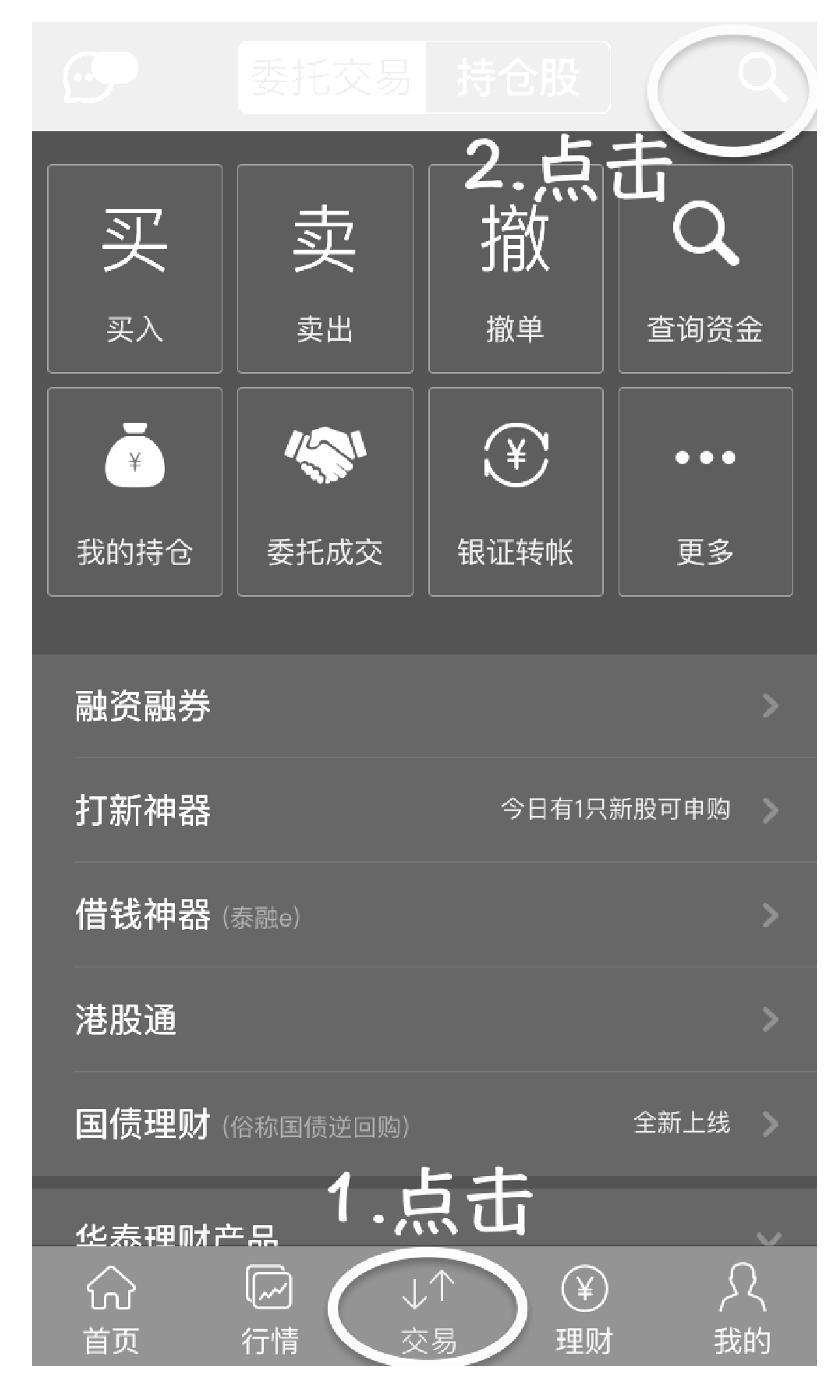
\includegraphics[width=0.45\textwidth]{figure/图13.1.png}
\caption{买入红利ETF步骤一}\label{fig:13-1}
\end{figure}

第二步，在查询框中输入“510880”，ETF的意思是交易型开放式指数基金，是场内基金的一种。点击该条目，进入510880的页面。

\begin{figure}[htbp]
\centering
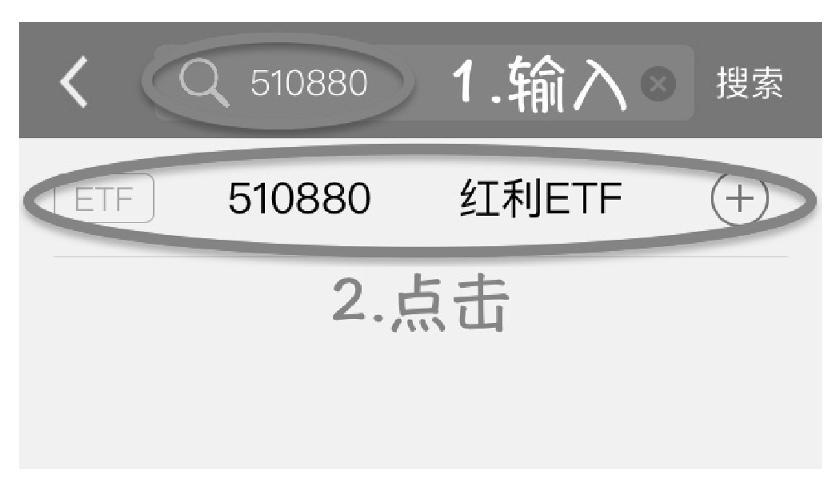
\includegraphics[width=0.9\textwidth]{figure/图13.2.png}
\caption{买入红利ETF步骤二}\label{fig:13-2}
\end{figure}

第三步，点击左下方的“买”，进行买入操作。

\begin{figure}[htbp]
\centering
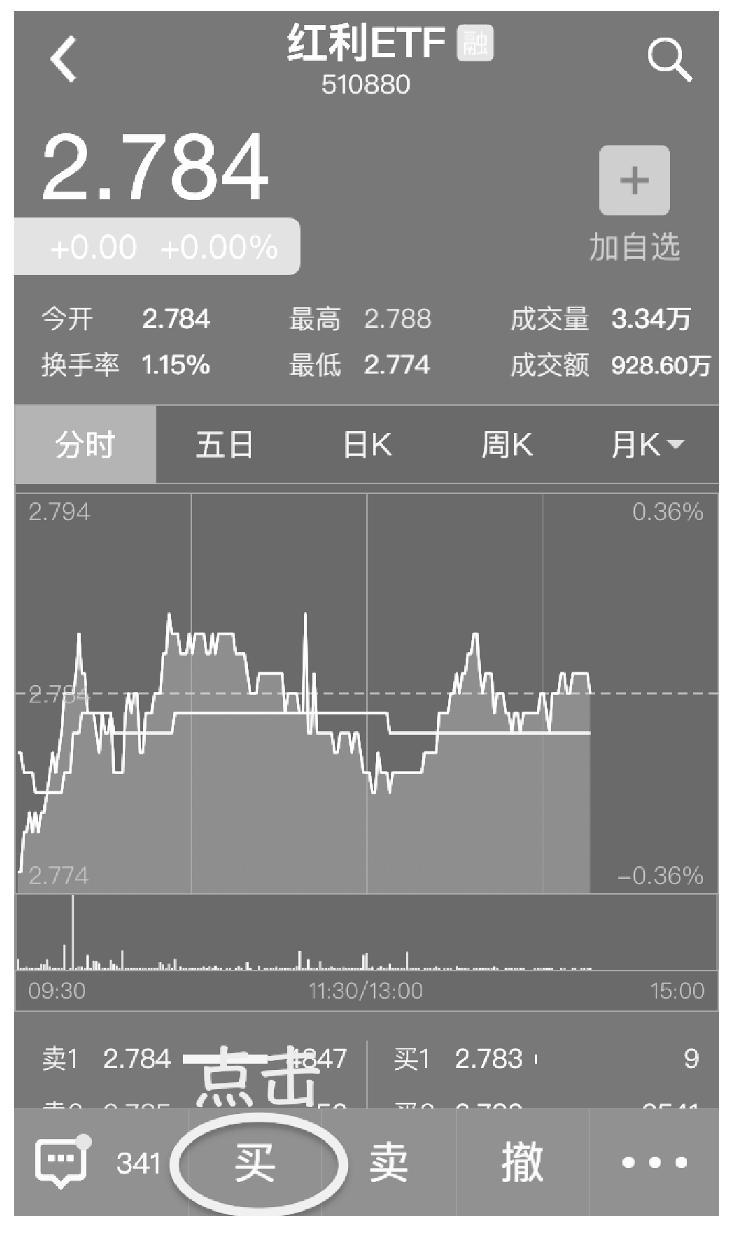
\includegraphics[width=0.45\textwidth]{figure/图13.3.png}
\caption{买入红利ETF步骤三}\label{fig:13-3}
\end{figure}

第四步，在买入页面中，输入准备买入的价格和份额。一般情况下，价格是自动输入好的，等于“卖一”的价格。在左下方可以看到，卖一价格为2.784元。

一般买入场内指数基金，填写“卖一”的价格；卖出场内指数基金，填写“买一”的价格。

填入价格之后，再输入买入的股份数，如200股。点击买入。场内交易是100股起买的，输入时也只能输入100的整数倍。大多数场内基金的单价在0.8～3元，所以只需要几百元就可以开始投资场内基金，门槛并不高。

\begin{figure}[htbp]
\centering
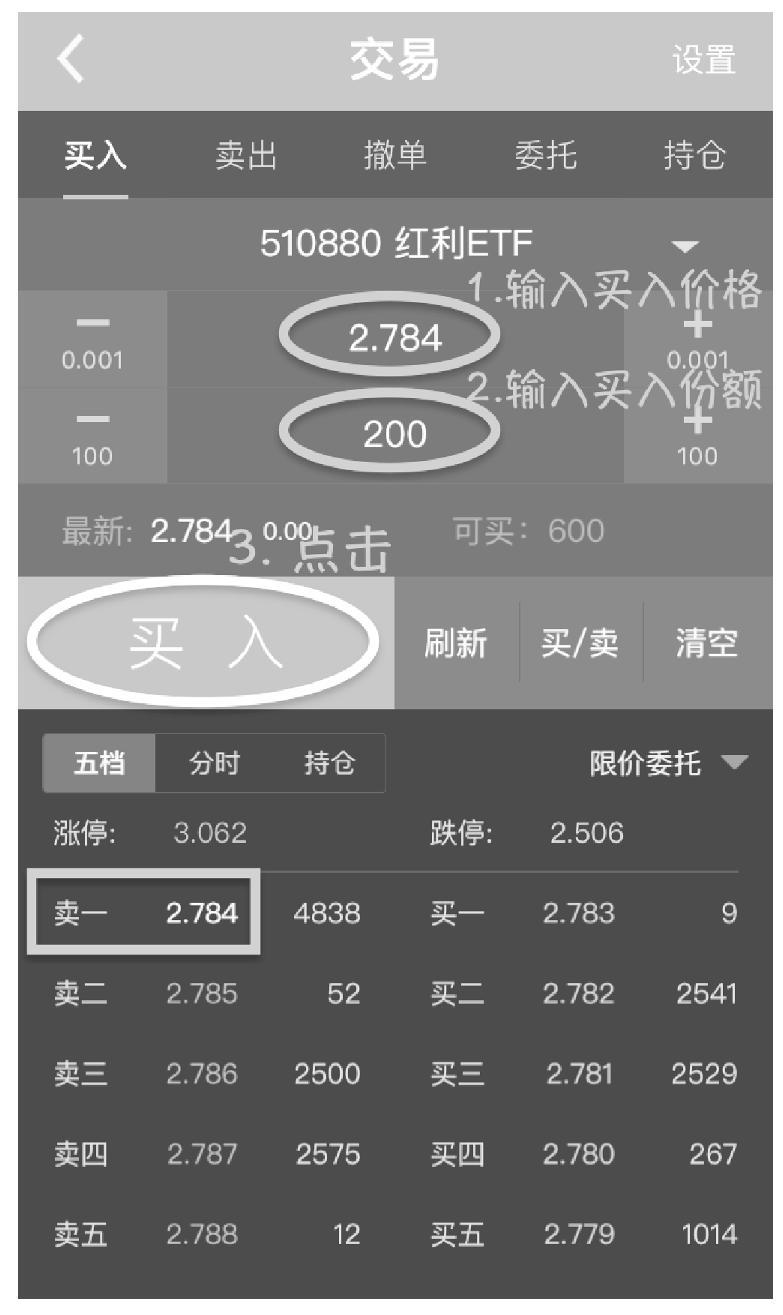
\includegraphics[width=0.45\textwidth]{figure/图13.4.png}
\caption{买入红利ETF步骤四}\label{fig:13-4}
\end{figure}

第五步，点击买入后，有一个弹出窗口，要求确认买入的基金代码和份额，点击确定后，系统会弹出提示，显示“委托提交成功”。这意味着成功提交了买入申请。但这并不意味着已经成功买入了，还得检查是否成功成交了。

\begin{figure}[htbp]
\centering
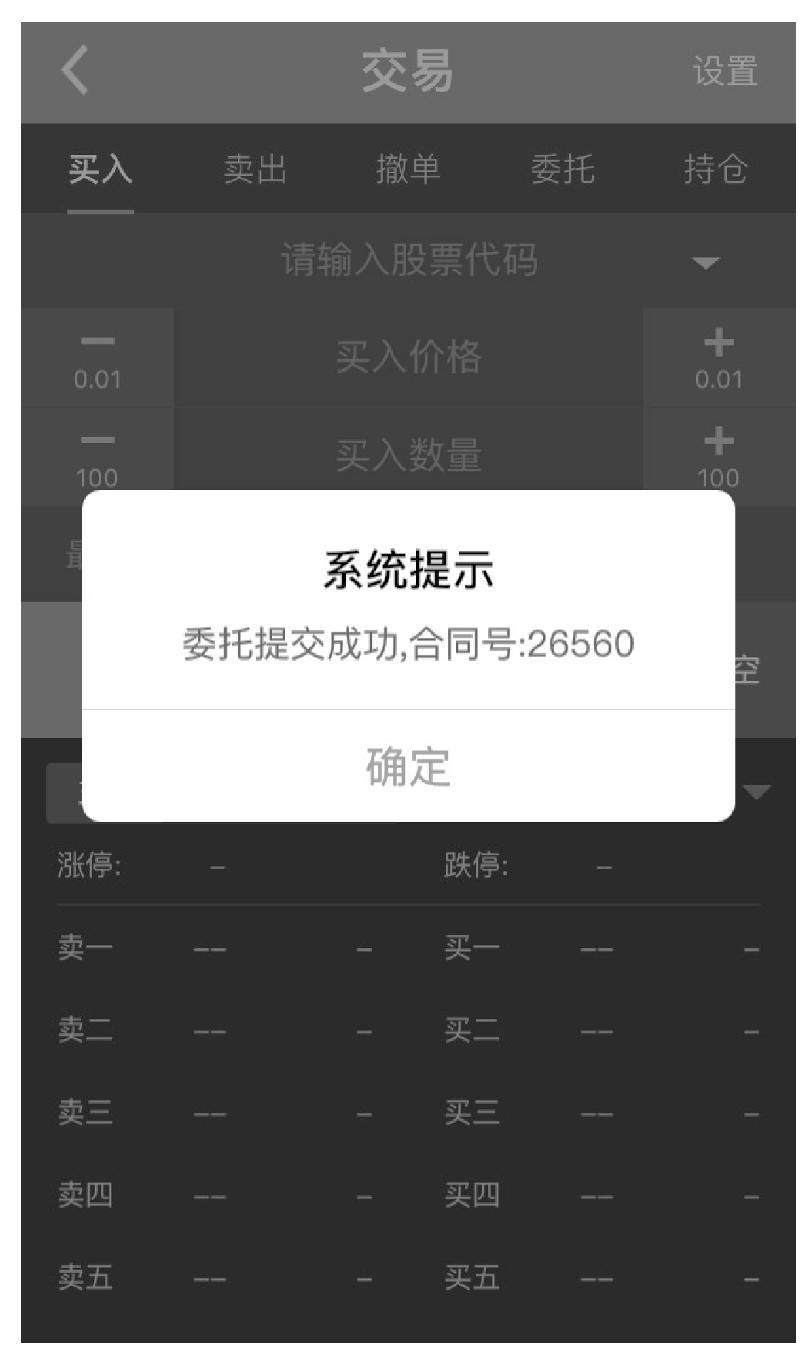
\includegraphics[width=0.45\textwidth]{figure/图13.5.png}
\caption{买入红利ETF步骤五}\label{fig:13-5}
\end{figure}

第六步，屏幕上方的几个栏目，分别是买入、卖出、撤单、委托、持仓等，点击“委托”，检查一下是否成功成交了。可以看到当日委托后面标注着“已成”，这就表示已经成功买入了200股红利ETF，成交价格为2.784元。

\begin{figure}[htbp]
\centering
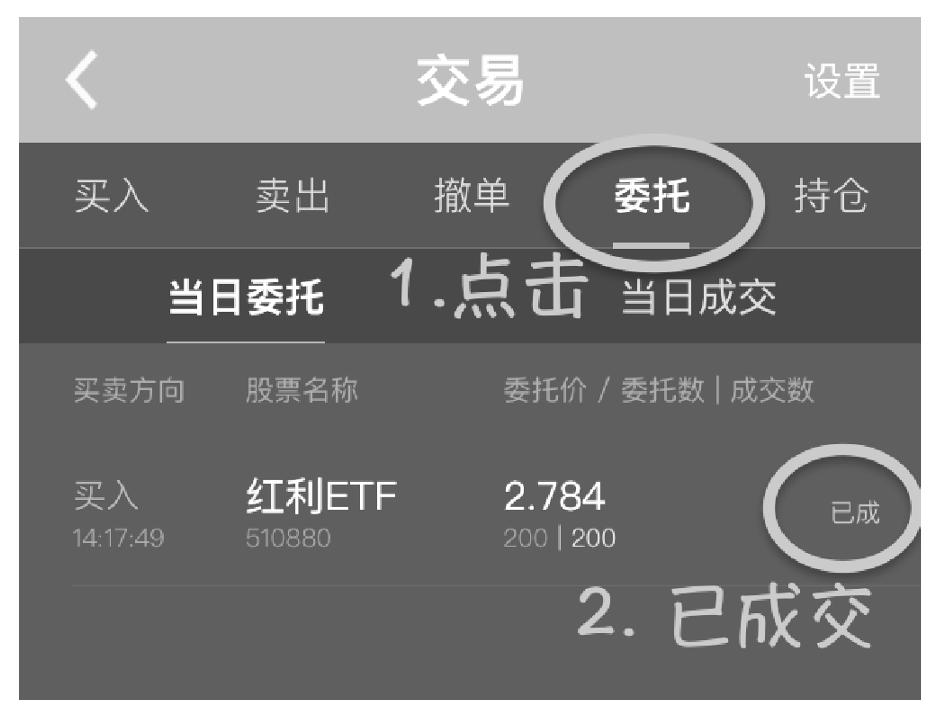
\includegraphics[width=0.86\textwidth,height=0.42\textheight,keepaspectratio]{figure/图13.6.png}
\caption{买入红利ETF步骤六}\label{fig:13-6}
\end{figure}

卖出基金的步骤与买入类似，不过选择的是“卖出”这一项进行操作。

（2）场外渠道的定投步骤详解。

场外渠道有很多，投资者可以在银行申购，也可以在基金公司的网站上申购。最近几年随着智能手机的兴起，支付宝、微信、雪球等网络平台也逐渐完善了。现阶段最方便、费用最低的渠道，还是这些网络基金销售平台。在螺丝钉的微信公众号“定投十年赚十倍”回复“场外基金”可以查看具体介绍。

场外基金并不是即时交易，所以在时间上是允许我们随时提交交易申请的。但是，不同的提交时间，成交的时间和价格都会有所差异。国内股市的收盘时间是交易日的15点，基金的净值一般在当天15点之后更新。在交易日当天15点之前申购，是按照当天收盘后基金的净值来申购，如果在当天15点之后进行申购，则是按照下一个交易日收盘后的基金净值来申购。需要注意的是，如果在节假日的时候进行申购，如周五16点申购或者周六周日申购，都是按照下一个交易日的净值申购，这样我们的资金就白白闲置了两天，没有任何收益。如果遇到长假日，资金闲置的时间会更久。所以申购的时候，要尽量选择在交易日的15点之前。

场外基金的申购，可以通过银行柜台，也可以通过网络平台。一些大型的、知名度高的网络平台一般都不错。现在网络渠道申购场外基金已经非常方便了，可以很方便地在手机或者电脑上申购基金。

这里以螺丝钉经常使用的基金平台——蛋卷基金为例，配合投资中证红利这只指数基金来演示具体的交易操作步骤，其他网络平台的操作类似。

第一步，进入App后点击上方搜索框，查找想要申购的基金。

\begin{figure}[htbp]
\centering
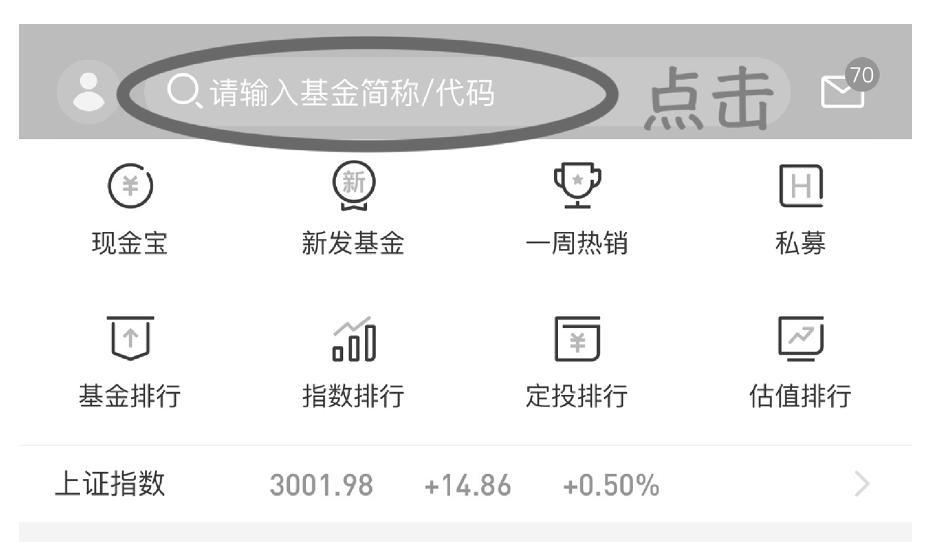
\includegraphics[width=0.86\textwidth,height=0.42\textheight,keepaspectratio]{figure/图13.7.png}
\caption{场外基金买入步骤一}\label{fig:13-7}
\end{figure}

第二步，在查询框中输入“100032”，点击“富国中证红利指数增强”。

\begin{figure}[htbp]
\centering
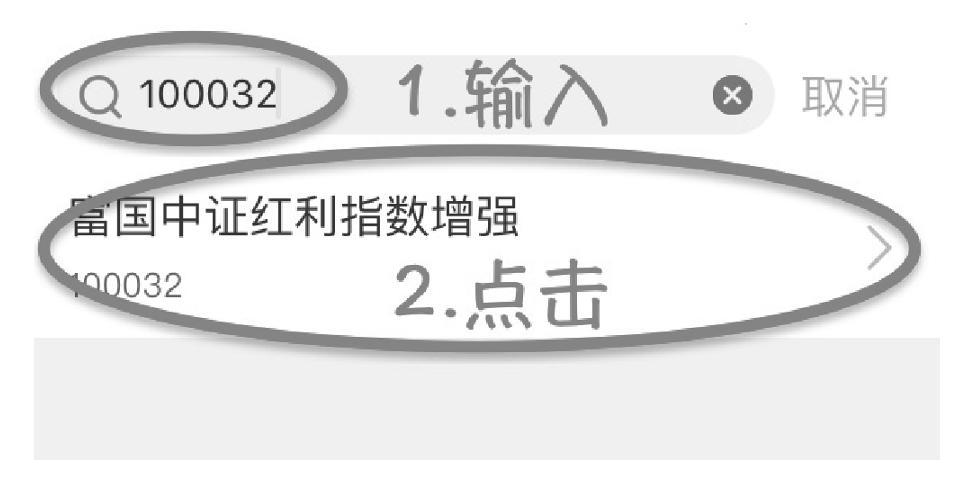
\includegraphics[width=0.86\textwidth,height=0.42\textheight,keepaspectratio]{figure/图13.8.png}
\caption{场外基金买入步骤二}\label{fig:13-8}
\end{figure}

第三步，进入基金页面后，点击右下角的“立即购买”。在“立即购买”的左边，还有一个“定投”，这是场外基金的自动定投功能，可以设置在固定的时间点由系统自动买入。

\begin{figure}[htbp]
\centering
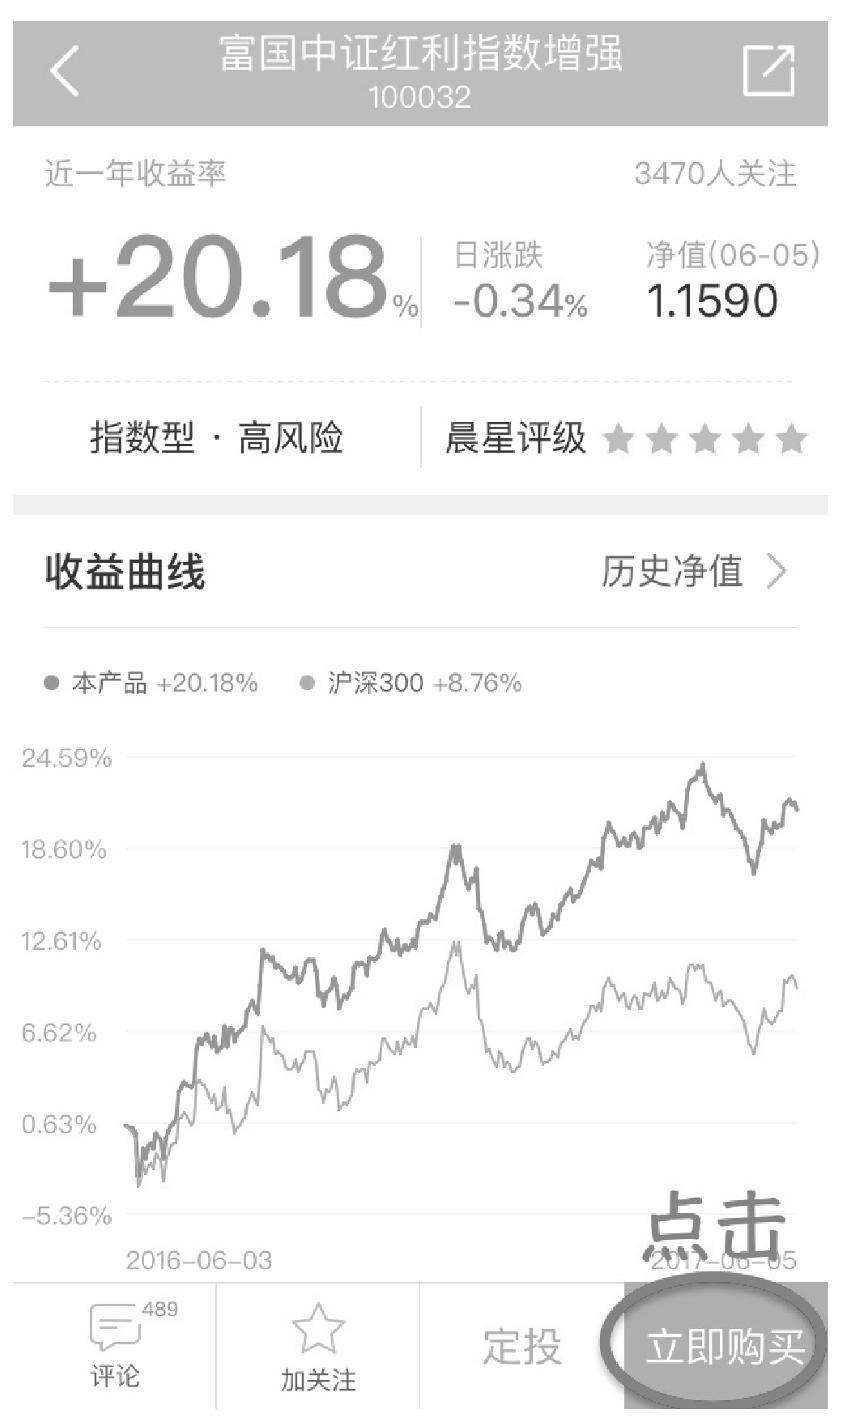
\includegraphics[width=0.58\textwidth,height=0.60\textheight,keepaspectratio]{figure/图13.9.png}
\caption{场外基金买入步骤三}\label{fig:13-9}
\end{figure}

第四步，输入准备申购的金额，比如1000元。场外交易基金时一般会有提示何时交易成功、何时开始计算收益、费率是多少等信息，在操作时注意看一下。输入金额后，点击“确定买入”，就完成买入操作的全部步骤了。

\begin{figure}[htbp]
\centering
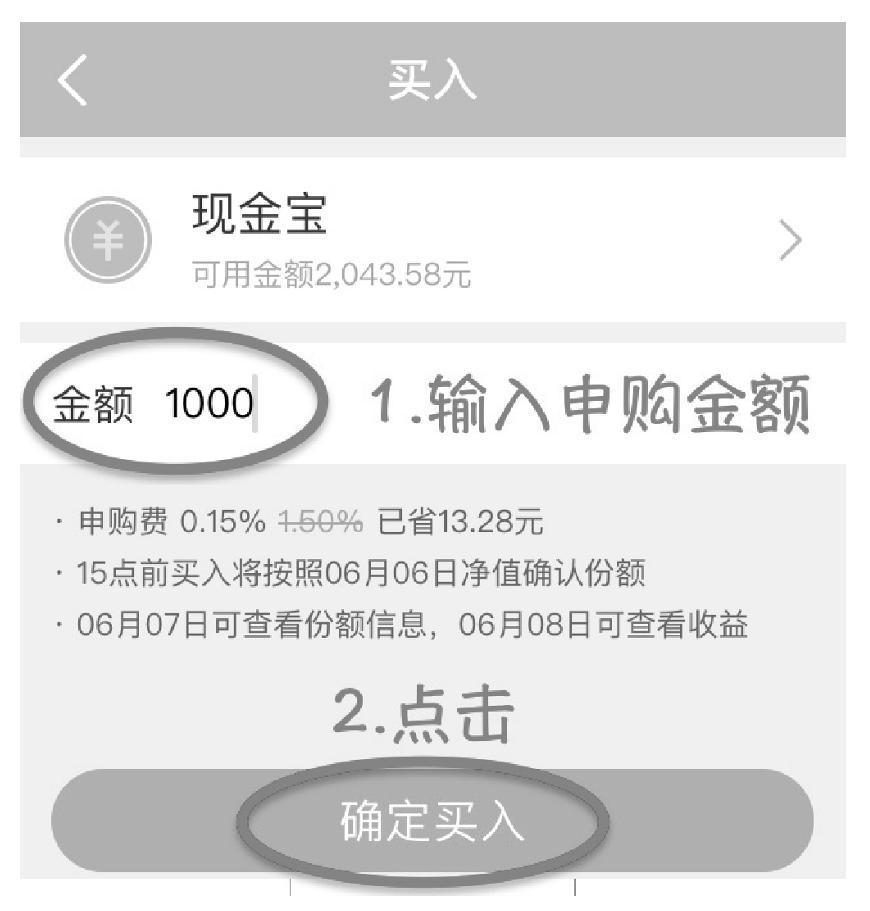
\includegraphics[width=0.72\textwidth,height=0.48\textheight,keepaspectratio]{figure/图13.10.png}
\caption{场外基金买入步骤四}\label{fig:13-10}
\end{figure}

场外基金的赎回操作也类似，不再赘述。

对于场外基金的申购赎回，有两点事项是需要注意的。一是尽量选择在交易日的15点前申购，以免造成资金闲置。二是申赎费率的问题。申购费是免不了的，但赎回费根据持有基金份额的时间长短而不同。一般持有基金份额不到一年的赎回费率是0.5\%，持有一年到两年的赎回费率是0.2\%～0.3\%，持有两年以上则没有赎回费。本书中介绍的定投指数基金的方式，一般会持有三年以上，所以赎回费基本上会省掉。

我们可以看到，场外的申购赎回在操作步骤上比较简单，新手容易掌握，但交易时间慢，不是即时交易。场内交易在操作界面上复杂一些，步骤稍多一些，但交易速度快，当时就能看到交易结果。场内渠道无法自动定投，需要手动定期买入来实现定投，而场外渠道有自动定投和手动买入两种方式，不过结合上一章介绍的“在低估的时候定投指数基金”，大多数时候我们也需要通过手动买入来实现这种投资理念。虽然手动定投麻烦一些，但能取得更好的效果。

\subsection{已经有一笔资金，要分批投入吗}
{\kaishu 手里有一笔钱，例如有50万元，是一次性买入便宜的指数基金，还是分批投入，或者是继续等待未来出现更便宜的价格呢？}

其实这个问题背后的回答，反映了你对市场未来走势的一个预判。

如果你愿意一次性买入，这说明你认为当前价格就是处于最底部，未来不会大幅下跌了。毕竟谁都想买在低点，如果未来还会继续下跌，没有人愿意现在就全部投进去的。

如果你想分批投入，例如分成10份，每个月固定买一份，这说明你持有的是被动投资的理念。“我也不知道未来是涨是跌，但只要还处于低估值，我就可以分批投入，最后的平均成本也一定是处于低估值的。”这样不会买在最低点，但也绝对不会买高。

如果你想持有现金，等待更便宜的价格出现，这说明你认为未来市场还会下跌。因为如果认为未来股价很快会涨上去，你不会现在持有现金的。这也是一种主观判断。

上面三种策略，只有分批投入是没有主观判断的。一次性投入和持币观望，都是对未来市场走势做出了主观判断。

如果主观判断正确，能赚到更多的钱；但如果判断错误，则有可能遭受损失。例如，持有现金等更低的价格，如果之后上涨了，就有可能踏空。

我们能大致判断出指数基金是便宜还是贵，但短期的涨跌是很难判断的。并不是说贵了短期就一定会跌，便宜了短期就一定会涨。

很少有人能长期准确地判断市场走势。我们定投的主要目的就是避免主观判断出错。分批投入至少可以获得一个平均价。只要每次买入都在低估值区域，最后的平均价也一定在低估值区域。能做到这一点，收益其实就已经有保障了。

这就是我们定投的意义：承认自己无法判断市场的走势，避免主观判断，用分批投入的方式来降低风险。

如果不是用新增的收入来定投，而是自己原本就有一笔资金，那该如何配置进去呢？

也可以用分批投入、越跌越买的方法。通常是把资金分成20份，进入低估区域后，投入1份，也就是5\%。这里的5\%，有点类似前面介绍定期不定额定投时的初始定投金额，之后每个月投入一份，如果市场下跌了，可以提高投入的比例和金额。用这种方式，可以在10～20个月里，把一笔资金分批配置成低估指数基金。

为什么是20个月呢？

这是一个经验数字，指数基金在熊市进入低估区域的时间长度平均为1～2年，历史最长也不过3年。但对一只指数基金来说，熊市低估的持续时间一般是1～2年。20个月是比较适中的一个时间长度，方便在熊市的资金配置，也不会让资金闲置太长时间。

投资者也不用担心，资金投入完成之后没钱定投怎么办。因为每一笔资金都是买入低估的指数基金，所以全部资金也都是买入低估的指数基金，整体买得仍然很便宜，长期收益就会有保障。

用这种方式，一笔资金也可以完成在熊市低估买入。

\subsection{日定投、周定投和月定投，哪种频率更好}
{\kaishu 日定投、周定投、月定投，哪种最好？分别适用于哪些不同的情况？}

经常有朋友问我定投频率的问题，是按周定投好，还是按月定投好。

定投的概念许多人都明白，就是定期投资，不过定投的频率就有多种形式了，有人按日、有人按周、有人按月，还有人随心所欲。

按日过于频繁，一般按周或者按月就好。假设每个月定投的资金量差不多，那这两种哪种更合适呢？

回测一下按周定投和按月定投的收益差距。一般定投时间越短，按周和按月收益差距就会越大。因为定投的时候如果赶上大跌或者大涨，就会对定投成本价产生很大影响。定投时间越短，造成的影响就会越大一些。但是定投时间越长，两者差距就会越小，定投达到5～7年时两者差距不到1\%，几乎可以忽略。所以从收益角度，定投频率影响不大。

不过从心理角度，这两种定投方式还是不一样的。按月定投比较适合大多数人，每个月发工资后买入，之后不用太操心，这种定投方式比较省心省力。不过有的投资者对下跌比较敏感，看到下跌就想多加仓，很难等待一个月之后再定投，这种投资者最好就按周定投。这样即使性子比较急，等一周的时间也应该没问题。

怎么知道自己是不是急性子呢？

其实判断方法也很简单：定投之后，如果看到下跌就买入，导致把下一次定投的资金提前投完了，最好就提高定投频率，按周定投，如果投完之后心安理得，就可以按月定投。

不建议根据自己的感觉来确定买入基金的时间。主观的感觉很容易受到市场波动的影响，遇到大跌或者大涨的时候，很容易就不敢买或者提前买的比较多，这样效果反而不好。而且从心理学的角度，人们对于同样数量的损失和盈利的感受是不一样的，损失带来的痛苦是盈利带来的喜悦的两倍至两倍半。换句话说，从情感上，赚200元得到的喜悦才抵得上亏损100元带来的痛苦。有这种影响在，主观的判断很容易不知不觉受到影响。所以最好是定期投资，而不是凭感觉来决定买入时机。

\subsection{定投一定能够降低成本吗}
{\kaishu 钉大，之前您不是说下跌时，加大投资额就会降低成本吗？那至少要提高多少投资额呢？为什么我每次加大投资额都没发现成本下降呢？}

如果出现这种情况，我们就要学习一个新的概念了：钝化效应。

定投有一个“钝化效应”。比如说，我们每个月定投1000元，坚持定投40个月后，会投入40000元的资金，也持有四万多元的指数基金。这个时候，如果我们再每月定投1000元，就会发现，增加的资金对原本持有的指数基金影响不大了。因为1000元对于四五万元的指数基金来说，占比太小了，影响也就很小。这就是钝化效应。

那么，钝化效应会发生在什么时候呢？

通常来说，如果你定投的资金额在你现在持有的指数基金总市值的5\%以下，那就接近钝化效应了。换句话说，如果每个月定投同样的钱，那么通常定投超过20个月之后，钝化效应就开始出现了。时间越长，钝化效应就越明显。

相反地，如果你这次定投的资金额在持有的指数基金总市值的5\%以上，那么对指数基金的成本还是会有比较大的影响的，这种情况下钝化效应不明显。

钝化效应对我们的投资会产生什么影响呢？

比如说，每个月定投1000元，定投了40个月，持有了四五万元的指数基金。这个时候，如果遇到大跌，如果我们投资的还是1000元，那么对于想要“降低持有成本”的效果就会差一些，因为1000元对四五万元的指数基金影响太小了。

不过，钝化效应对收益率的影响不大。它主要是让我们持有指数基金时的波动增加。原本没有钝化效应时，定投可以降低波动，但是钝化效应出现之后，定投降低波动这个效果就减弱了。

为了降低钝化效应，我们就需要改变定投的金额。这也就是“定期不定额定投”方法的原理。

现实生活中，我们可以直接采取一种非常简单、不需要复杂计算的方式，那就是：固定拿出工资的一定比例来定投。这样做能够在一定程度上缓解钝化效应。因为工资通常是会随着时间长期上涨的，所以定投的金额也会随着工资的增长而不断增加。

另外，当我们遇到指数基金下跌时，还可以采取“越便宜，定投买入越多”的方式来缓解钝化效应。这种方式需要我们根据指数基金当前的估值，来计算这期应该定投的金额。具体的计算公式参照本书第10章的内容。

另外，每次当指数基金进入高估区域的时候，我们会分批卖出，得到的资金再分批投入当时其他低估指数基金，这样就盘活了存量，钝化效应就消失了。

\subsection{定投多久，才能开始赢利}
{\kaishu 我们定投指数基金，是不是需要很久才能赚到钱呢？大概定投多久能开始赢利呢？}

这个问题是很多朋友非常关心的问题。

过去4年，基本上每年都有低估的品种出现。我们在2014、2015、2016、2017年，每年定投的收益都不错。这4年里，基本上从定投低估品种开始到赢利，都不到1年时间。最长的话，是需要定投两年多开始赢利。也就是2012—2014年，A股史上最大的一次熊市，这次熊市要定投两年多才开始赢利，但大多数都不需要这么长时间。

如果是这两年开始定投的朋友，账面上可能会有10\%～15\%的浮亏（截至2019年5月31日）。不过，如果是在2016年定投低估品种，到目前还是正收益的，例如H股、恒生指数基金，更不用说在2014年熊市投入的品种。

假如说A股保持2600～2700点不变，不涨不跌，我们大概定投多久开始赢利呢？

以中证红利指数为例，它的盈利增速还可以，长期来看仍然能保持10\%的增速。

\begin{itemize}
\item 2019年：市盈率达到7.4倍，股息率为4.4\%。
\item 2020年：市盈率达到6.7倍，股息率为5\%，这已经接近中证红利指数历史最低估值了。
\item 2021年：市盈率达到6.1倍，股息率为5.3\%。
\item 2022年：市盈率达到5.5倍，股息率为6\%。
\item 2023年：市盈率达到5倍，股息率为6.4\%。
\end{itemize}

可以看到，假如A股保持2600～2700点不变，那么未来两年，从中证红利指数上，单单是分红收益的积累，就接近10\%了，而且还会越来越高。

定投有摊低成本、减少浮亏的效果。大部分2019年定投的朋友，坚持定投下来，浮亏会在10\%～15\%。继续定投，浮亏还会进一步减少。

也就是说，在低估区域定投两年，假设股价不涨不跌，我们单靠“定投+分红收益”也可以弥补大部分亏损。

其他的低估品种也是类似的原理。很多品种目前的估值也处于自身估值的最低区域。未来指数背后公司的盈利上涨，也会推动指数上涨。

股价不可能一直保持不变。只要股价稍有上涨，我们的定投开始赢利是很容易的。

所以坚持定投，大概率在未来1～3年开始赢利。通常1年多就开始赢利。

因为指数基金的波动有一定范围，但指数基金背后公司的盈利是长期增长的。

其实这些道理，大部分朋友也都明白，真正难的是坚持定投。

就像锻炼，刚开始的那段时间，浑身肌肉酸痛，痛不欲生，但是只要咬牙坚持渡过了这段时间，之后就轻松了。

定投也是如此。开始经历熊市的时候，是比较难受的。只要坚持完一轮牛熊市，之后的长期投资就没有太大的障碍了。从知识，到经验，再到心理素质，就真正成熟了。

耐心，是投资者最好的美德。

\subsection{看点数来买基金，靠谱吗}
{\kaishu 指数的点数有什么用？为什么一个指数在同样点数的情况下，有的时候适合投资，有的时候却不适合投资呢？}

螺丝钉有个爱好是看旧书，以前看过一些十几年前的基金类书，其中有一个策略说：“在上证指数1500点以下买基金，到了2500点就卖掉。”

像这样看点数来买基金的策略会有效吗？

我们都知道指数是有点数的，例如上证综指接近2800点，恒生指数接近28000点等。

这个点数代表什么呢？

我们可以简单地理解为：点数就是指数中所包括的成份股的平均价格。如果指数包括的成份股的股价平均上涨了1\%，那么指数的点数也会随着上涨1\%。一般每个指数都会有一个起始点数。比如上证综指和恒生指数，都是从100点开始的。

为什么是100呢？

这是人为指定的。指数公司会统计一下指数开始的那一天，股市上所有股票的总股价，并把这个总股价设置为100。当然了，也有的指数是从1000开始的。

之后，如果整个股市上涨1\%，指数的点数也会上涨1\%；如果整个股市下跌1\%，指数的点数也会下跌1\%。

从这个角度，我们就可以更方便地理解指数点数的意义了。

例如，恒生指数从20世纪60年代的100点涨到了今天的约27500点，上涨了270多倍。上证综指，从1991年的100点涨到了今天的约2800点，不考虑分红收益也上涨了28倍。

未来，上证综指也会像恒生指数一样，从上涨28倍到上涨280倍，但还是需要时间的。A股的历史还比较短。

为什么指数的点数会长期上涨呢？

点数可以看作指数中包含股票的平均股价，那我们可以把它分解一下：

{\kaishu 股价=（股价/每股盈利）×每股盈利=市盈率×每股盈利}

这就是市盈率的定义了：

{\kaishu 市盈率=股价/每股盈利}

市盈率是最常使用的一个估值指标。

只要公司的盈利是正常的，我们就可以计算它的市盈率。

指数包括了一篮子的股票，所以指数从整体上来看也是有一个总盈利的。我们用指数成份股的总股价除以总的盈利，就能得到指数的市盈率。市盈率的变化是有范围的。

我们可以看一下，在过去几十年的历史中，恒生指数的市盈率变化，如图 \ref{fig:13-11} 所示。

\begin{figure}[htbp]
\centering
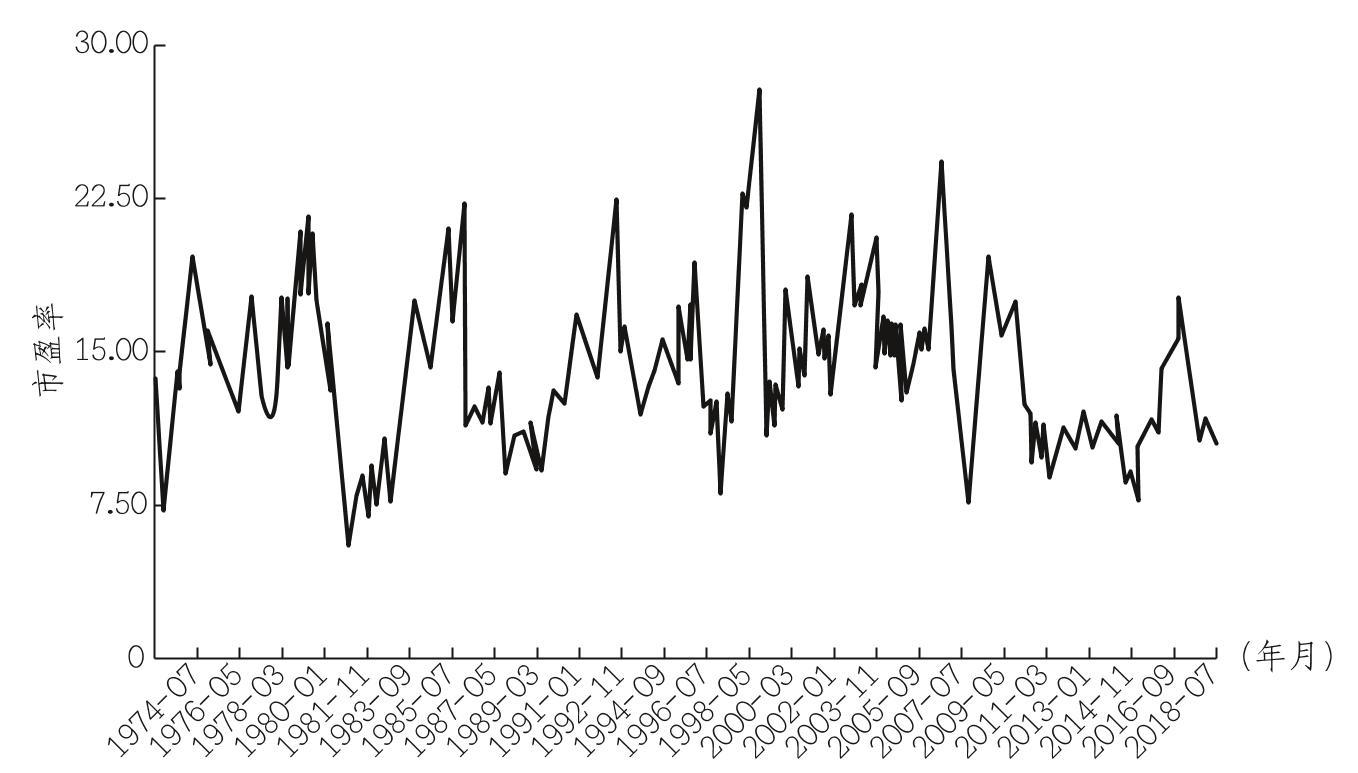
\includegraphics[width=0.90\textwidth,height=0.40\textheight,keepaspectratio]{figure/图13.11.png}
\caption{恒生指数的市盈率变化}\label{fig:13-11}
\end{figure}

恒生指数的市盈率最低到过5倍左右，最高到过28倍左右，估值是有极限的。其他时间里，恒生指数的市盈率主要集中在10～20倍左右。

其实，恒生指数从创立之初到现在，市盈率甚至变小了，从30多倍到了10倍左右。

那么，问题来了，市盈率变小了，为何点数还能上涨280倍呢？

最主要的原因，就是盈利的增长。恒生指数背后公司的整体盈利是长期上涨的。

科技的进步、管理效率的提升、生产力和生产效率的不断进步，都使企业整体的盈利上涨。虽然在短期某几年内可能会遇到一些经济危机，如亚洲金融危机、美国次贷危机等，但是总体来看，企业的整体盈利长期是在不断向前进步的。

正是盈利的长期上涨使指数的点数能够长期上涨。

虽然指数长期是上涨的，但是在短期内还是会暴涨暴跌的，这种暴涨暴跌主要是受到了估值的影响。

像2015年年初至2015年6月这段时间，A股指数的盈利并没有大幅上涨，但是指数的点数大幅上涨了。这就是因为大量投资者都看好股市，大量的资金涌入导致估值提升。

如果投资者在估值高点买入，那么之后遭遇大幅下跌就在所难免了。

最惨的情况就是像20世纪80年代末的日本股市：整体估值特别高，同时实体经济也有泡沫。一旦泡沫破裂之后，指数的整体盈利下降，估值也从高点下降，指数遭遇双重打击。这种情况下，指数就很难在短期内恢复了。所以日本指数当年创下接近4万点的高峰，结果快30年过去了，还只有两万点左右。

所以，“买指数就是买国运”这句话非常有道理，国家经济的长期发展是指数盈利不断上升的保障。

投资指数基金，首先，要对这个指数背后的国家有信心，其次，为了避免长达七八年甚至十几年的浮亏，我们要在指数低估的时候分批买入。这样，既可以享受指数长期盈利的上涨，又避免了短期的大幅下跌。

看点数来买基金的策略，是一个“刻舟求剑”型的策略。

港股恒生指数，以前也曾经在一两千点徘徊，但是随着长期上涨，今天已经到两万多点。所以，看点数来投资的策略就失效了。

A股的整体盈利，长期来看是不断上涨的。A股指数，从1991年的100点涨到现在的2700点，以后还会逐渐提升的。每隔10年，这个点数都会跟之前有很大的不同。

看点数来投资，可能在短期内会有一定效果，但是长期来看，迟早会失效的。

\subsection{有没有完美的“高抛低吸”投资方法}
{\kaishu 有没有更好的牛市卖出方法？是不是存在一种完美的卖出方法，能够让我们每次获得上涨的收益，还能够完美地避开之后的下跌呢？}

我要给大家“泼一盆冷水”：不存在这样的方法。

我们先假设存在这样的方法，并且可以学习到。

国内偏股型混合基金的整体历史走势如图 \ref{fig:13-12} 所示。

\begin{figure}[htbp]
\centering
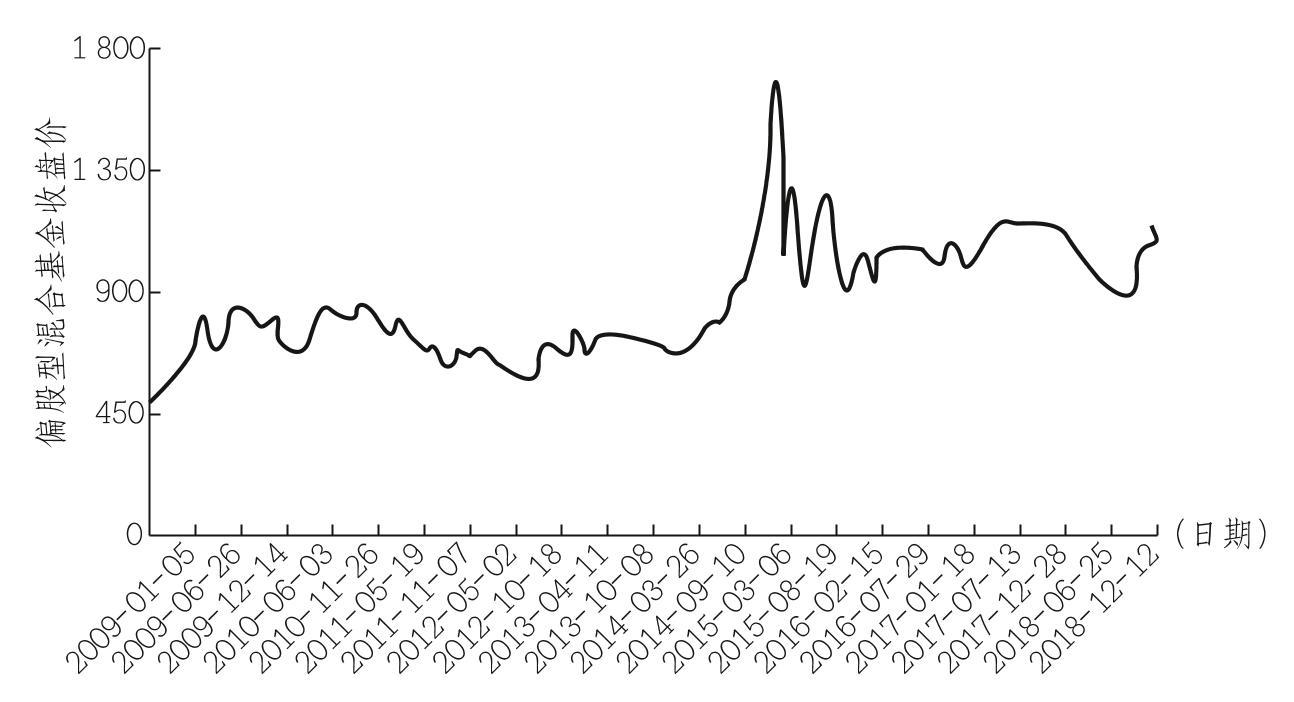
\includegraphics[width=0.90\textwidth,height=0.40\textheight,keepaspectratio]{figure/图13.12.png}
\caption{国内偏股型混合基金的整体走势}\label{fig:13-12}
\end{figure}

偏股型混合基金是什么呢？

我们平时说的指数基金，是一种股票基金。指数基金不管什么时候，基本都会持有90\%以上的股票仓位。混合基金则是股票和债券都有。像偏股型混合基金，主要是投资股票，不过它的股票仓位最低可以到50\%。换句话说，如果混合基金的基金经理觉得股市有风险，可以主动把股票仓位降下来。目前国内有500多只偏股型混合基金。

如图 \ref{fig:13-12} 所示，偏股型混合基金的最高点在2015年6月。股灾发生后，偏股型混合基金大幅下跌，到了9月下跌近38\%，同期沪深300指数下跌了30\%。这说明了什么呢？

混合基金都是主动型基金。

混合基金的基金经理的从业要求大多是“国外金融学硕士或者博士，有多年从业经历”，他们无论是在知识储备还是投资经验方面，都是所有投资者中万里挑一的（国内有3亿多投资者，而公募基金的基金经理人数只在万人级别，绝对的万里挑一）。

他们只要在牛市高位的时候，下调混合基金的股票仓位，从股票换到债券，就可以保住之前牛市的收益、避开之后的股灾。不仅基金净值收益好，自己也可以获得更高的业绩提成和奖金。但是很遗憾，从混合基金的整体表现上来看，这些混合基金几乎都没有减仓股票。换句话说，这些顶尖级的投资高手也没能精准地判断牛市拐点。

如果真的存在这么一种能精准判断牛市拐点又长期有效的方法，并且可以通过学习获得，那么这些基金经理绝对有动力、有条件去学习并实践的。不过从事实上来看，这样的方法并不存在。

股市的短期走势是无法预测的。

美股曾经有一个很著名的预测指标，叫作“超级碗指标”（Super Bowl Indicator）。美国人很喜欢看橄榄球比赛。曾经有人发现，如果美国国家橄榄球联合会（NFL）的队伍赢了，股市下一年会平均上涨14\%；如果美国橄榄球联合会（AFC）的队伍赢了，股市则会平均下跌10\%。

从1967—1997年，在这长达30年的时间里，有28年都是如此，很多人都对这个方法深信不疑，并赚到了很多钱。

但是从1998年开始，这个方法失效了。在之后的很长时间里，甚至跟之前的情况完全相反，这让很多通过比赛结果预测股市的投资者损失惨重。

之所以会出现这样的情况，是因为股市的短期走势无法预测。在漫长的历史上，总会有一段时间的股市走势恰好跟某个指标非常匹配，好像这个指标可以预测短期走势，但当时间拉长了，这个指标就会失效。所以通过绘制历史趋势线来预判未来走势，可能一段时间内会成功，但长期来看必然会失效。

但是股市的长期走势是有迹可循的，原因在于股市的复利效应。

股票资产是有复利的。公司每年会把盈利的一部分再投入生产，以便来年产生更多的盈利，也会将盈利的一部分以现金分红的形式发放给股东。这都会推动股市整体上涨。所以我们看到，股市指数整体是上涨的。美股百年里上涨了200多倍，港股53年里上涨了600倍，A股从1991年至今也上涨了30倍。

估值低并不意味着短期会上涨，但是估值越低，3～5年以上的收益就会越高。这个理论得到了许多投资大师的印证。

（1）格雷厄姆等人的研究表明，在低市盈率的时候投资，能带来更好的收益。

（2）1991年美国基金经理迈克尔·奥希金斯提出的“狗股理论”表明，股息率越高，长期收益率越高。

（3）1992年，尤金·法玛等人的研究表明，低市净率也能获得高收益。

这些大师的投资结论，无一例外都是建立在几年甚至十几年以上的时间跨度上的。低估值投资也是一个长期坚持才能体现出效果的策略，并不是短期里的预测指标。

总结一下，股市短期走势无法预测，但直到今天仍然有很多投资者不相信这一点，试图寻找完美的“高抛低吸”的短线技巧。不过股市的长期走势有迹可循，特别是3～5年或5年以上的收益，跟估值有很强的相关性。买入估值越低，长期收益越高。

\subsection{定投低估的指数基金，最大浮亏是多少}
{\kaishu 钉大，按照你的基本思路执行定投，就是每月定额买低估值的品种。期间出现极端熊市，比如2012、2013年，账面可能会浮亏多少？有没有一个大概的测算呢？}

我们在投资低估指数基金的时候，要明白的一点：低估并不代表不再下跌。而是，当前处于低估的指数基金，具有很不错的投资价值。因为低估和高估都是一个区域。既然是一个区域，那在这个区域里就会有上涨和下跌。

很多朋友在投资的时候，容易犯的一个错误是：总想着能够买在最低点、卖在最高点。

比如，螺丝钉经常会被问道：“既然当前下跌了这么多，那前段时间先不投，等到现在再开始投资不是更好吗？我之前都买贵了。”“如果指数进入高估之后我们就开始卖了，比如4000点就开始卖，那后面继续上涨到5000点、6000点，我们岂不是得不到最高的收益吗？”

其实，如果总想买在更低点，那我们可能等到的投资机会就比较少，无法积累足够多的份额。没有足够的份额，即使将来收益率再高，也无法解决我们的实际问题。

而如果总想卖在最高点，那我们可能需要承担更大的风险。

因为最高点之后，紧接着可能就是大幅的下跌。我们可能为了多赚10\%要承担之后“腰斩”的风险。“君子不立危墙之下”，没必要赚最后一块硬币。

那么，低估的指数基金的最大跌幅是多少呢？

其实不同类型的投资品种，在熊市低估区域，波动范围会有区别。

如果是包含多种行业的宽基指数，在熊市低估区域，跌幅通常为20\%～30\%。如果是单个行业，波动会更大一些，跌幅为30\%～50\%。如果是单只股票，波动会更大，跌幅甚至超过50\%。

我们以2018年的熊市为例。2018年，是A股历史上的第二大熊市，沪深300指数跌幅大约为25\%，代表了主流指数的平均跌幅。

不过虽然指数下跌25\%，但如果定投的话，在微笑曲线的作用下，浮亏会大大减少。通常只有1/3～1/2的浮亏，也就是浮亏在10\%～15\%。

这就是定投宽基指数，在大熊市的浮亏情况。

我们通常不会一次性投入，而是配合分批定投的策略，通过定投的方式，在浮亏的时候摊低成本。

如果是用定期不定额的定投方法，也就是越低估买入越多，浮亏也会更小一些。

其他品种也是同样的道理。

所以，如果坚持定投低估品种，大部分品种在大熊市浮亏会在10\%～15\%。继续定投，浮亏还会继续减少。

定投可以摊低成本，让我们的浮亏减少（例如品种本身下跌20\%，定投可以让浮亏减小到12\%左右），之后不需要涨回到原来的位置，我们的盈利也会不错。这就是定投的“微笑曲线”。

我们要做的是在低估浮亏的时候尽量坚持定投，积累更多的股份。
